\chapter{Base Features}
\label{ch:base-features}

Let us first go through some of the base features offered by \LaTeX{} and used in
this template.
Before anything happens, the \TeX{} engine is chosen.
This is the binary responsible for compiling the \LaTeX{} source code.
If you have used \LaTeX{} before but never heard those terms before, you are most
likely using \hologo{pdfLaTeX} as your engine.
This is the go\-/to default for generating \abb{portable_document_format} output.
Its most popular modern alternatives are \hologo{XeLaTeX} and \hologo{LuaLaTeX}.
These two offer various new, shiny features, chief among which is Unicode
support through the package \ctanpackage{unicode-math}, which builds onto
\ctanpackage{fontspec} and extends it by capabilities for math fonts.
More on that in \cref{ch:fonts_text}.

\hologo{LuaLaTeX} is preferred over \hologo{XeLaTeX} for the following reasons:
\begin{enumerate}
    \item \ctanpackage{contour}, a package that can do things like
        \contour{black}{\textcolor{white}{this}}, works.
        For an application of that, see \cref{fig:bitmap_tikz} on
        \cpageref{fig:bitmap_tikz}.
        Getting \ctanpackage{contour} to work on \hologo{XeLaTeX} is somewhat impossible.
    \item \hologo{LuaLaTeX} allocates as much memory as it happens to need.
        The ancient limitations of \TeX{} are easily reached by packages like
        \ctanpackage{tikz} and \ctanpackage{pgfplots}.
        Circumventing that either feels hacky, or actually is hacky.
        \texttt{tikzexternalize} is a great module, but has a long list of caveats.
        It solves a problem that should no longer exist in the first place.
    \item The fantastic \ctanpackage{microtype} package has a number of unavailable
        functionalities when using \hologo{XeLaTeX}.
\end{enumerate}
Using \hologo{LuaLaTeX}, you do not have to worry about any of that:
hit compile, wait, done%
\footnote{
    The \emph{waiting} part might be a bit longer than what you might be used to
    from \hologo{pdfLaTeX}.
    So far, this is the only disadvantage I could find.
}.

\section{Fonts and Text}
\label{ch:fonts_text}

Using high-quality fonts is one goal.
This includes the fantastic
\href{https://ctan.org/texarchive/fonts/tex-gyre/opentype}{\TeX Gyre fonts},
of which the \textit{\href{https://en.wikipedia.org/wiki/Palatino}{Palatino}}
(by Hermann Zapf) clone \textit{\href{https://ctan.org/pkg/tex-gyre-pagella}{Pagella}}
was chosen for this document.
It comes with an accompanying
\href{https://ctan.org/texarchive/fonts/tex-gyre-math/opentype}{math font}
of the same name%
\footnote{
    Both fonts are vector fonts;
    if \LaTeX{} yields any warnings about \emph{font size substitutions},
    that is bogus and can be ignored.
}%
.
Using both fonts together is made possible by the \ctanpackage{unicode-math} package.
As such, an exact match of the text and math fonts is achieved.
This is important but often overlooked.
However, such a match is often plain unavailable in the typesetting tool at hand.
\LaTeX{} is no exception here if there simply exist no matching fonts.
We took care to ensure a complete match here.

Not only do the fonts look great on their own and paired up, they (just as importantly)
also feature very broad support for all sorts of symbols and characters, as well as font
shapes and weights and combinations thereof.
The latter is demonstrated in \cref{tab:main_font_examples}.
%
\begin{table}\ContinuedFloat*
    \ttabbox{%
        % Brackets hold entry that will go into List of Tables (short form)
        \caption[Main/Roman Font Examples]{%
            Examples for font features offered by the main roman font.
            Notice the small vertical white space after the fourth row,
            nicely separating content that is slightly dissimilar%
        }%
        % Use a string like 'tab:' to help with organization and auto-complete
        % when reffing
        \label{tab:main_font_examples}
    }{%
        \small
        \begin{tabular}{
            % @{<value>} specifies the column separator;
            % Use @{} to remove white space from sides (empty value)
            @{}
            l% If no other significant reason, left-align
            l
            @{}
        }
            \toprule
                Feature & Sample Text\\
            \midrule
                Regular & \sampletext\\
                \textbf{Bold} & \textbf{\sampletext}\\
                \textit{Italics} & \textit{\sampletext}\\
                \textbf{\textit{Bold Italics}} & \textbf{\textit{\sampletext}}\\
            % Some inconspicuous vertical separation,
            % more visually pleasing than a full rule
            \addlinespace
                \textsc{Small Capitals} & \textsc{\sampletext}\\
                \textbf{\textsc{Bold SC}} & \textbf{\textsc{\sampletext}}\\
                \textit{\textsc{Italics SC}} & \textit{\textsc{\sampletext}}\\
            \bottomrule
        \end{tabular}
    }%
\end{table}

Combine all that with \ctanpackage{microtype} (a package taking care of typesetting
details), and we get very beautiful typesetting.
For example:

\begin{displayquote}
    \blindtext
\end{displayquote}

Notice the balanced line endings and low number of hyphenation;
easy on the eyes and very readable.

\paragraph{Old approach}
The overwhelming majority of \LaTeX{} documents rely on the two lines
\begin{minted}[linenos=false]{latex}
    \usepackage[T1]{fontenc}
    \usepackage[utf8]{inputenc}
\end{minted}
This approach is \textbf{outdated} and only required when using \hologo{pdfLaTeX}.
Since this is what most people still do, the two packages are still required.
However, these two packages should at least not be used for \emph{new} work anymore!
Using \hologo{LuaLaTeX}, they are not required anymore:
\begin{itemize}
    \item input encoding is automatically UTF-8 (as it should be in 2020),
    \item font encoding is also not required, since fully capable fonts are used,
        which come with all the glyphs required.
\end{itemize}
The same is true for \hologo{XeLaTeX}.

\subsection{Math}

What often does not occur at first glance is that many documents use text and math fonts
that are very different from one another.
As far as I know, Microsoft's \emph{Word} has usable math typesetting and sensible default
fonts for that.
Yet, it cannot do what dedicated, fully\-/fleshed text and math fonts
--- different, but matched ---
can achieve.
They provide a seamless transition, especially when using actual text in the math
environment or vice versa, like when we go for \(x \to \infty\) and then also do
\(\int_{1}^{2} y^2 \deriv{y}\) or maybe \(a^2 + b^2 = c^2\).
All these inline math elements look perfectly natural.
If instead the fonts did not match, inline math would stick out like a sore thumb.
Toggle the colors in the class file (\texttt{*.cls}) to highlight each different
font family to see all the differences (see the \verb|Color| option for
\ctanpackage{unicode-math}).
Some display-style math examples follow.
\begin{gather}
        \sym{pressure}\symspec{volume}
        =
        \symspec{gas_constant}\sym{abs_temperature}
        \label{eq:glossaries_extra_example}
    \\
        \cons{euler}^{\cons{imaginary}\cons{pi}} + \num{1} = \num{0}
    \\
        \tcbhighmath{
            \lim\limits_{\sym{first_cart_coord} \to \infty}
            % Writing \frac this verbosely is good for readability and diffing/VCS.
            % This way, the fraction parts are stacked on top of each other, just like
            % they are in the print output.
            % Since math contexts gobble all whitespace anyway, we can freely use it
            % without accidentally producing extraneous spaces in the output.
            \frac{
                \cons{pi}\parens*{\sym{first_cart_coord}}
            }{
                \sym{first_cart_coord} / \ln\parens*{\sym{first_cart_coord}}
            }
            =
            \num{1}
        }
        \label{eq:highlighted}
    \\
        \sum_{\sym{count} = \num{0}}^{\sym{component}}
            \begin{pmatrix}
                \sym{count} \\ \sym{component}
            \end{pmatrix}
        =
        \num{2}^{\sym{count}}
    \\
        % This equation does not make sense.
        \brackets*{
            \sym{abs_temperature}
            \cancelto{\num{0}}{
                \fracderiv*{%
                    %
                }{%
                    \sym{abs_temperature}
                }
            }
            +
                \sym{ratio_of_specific_heats}\parens*{\sym{pressure}}
                \fracderiv*{}{\sym{density}}
            +
                \sym{angle_one}
        }
        \sym{celsius_temperature}^{\sym{count}}
        \parens*{
            \sym{first_cart_coord}_{\num{1}},
            \sym{first_cart_coord}_{\num{2}},
            \dots, \sym{first_cart_coord}_{\sym{count}}
        } = \num{0}
    \\
        \difference{\symspec{enthalpy}_{\text{change}}}
        =
        \nicefrac{\num{1}}{\num{2}}
        \parens*{
            \sym{velocity}^{\num{2}}_{\text{exit}}
            -
            \sym{velocity}^{\num{2}}_{\text{entry}}
        }
\end{gather}
If these symbols are colored, it is because they are links and link coloring is on.
This can be turned off (globally or for certain elements) in the options to
\ctanpackage{hyperref}.
If color is turned off, they are still hyperlinks.
If even that is undesired, that can also be turned off in that package.

\subsubsection{Predefined Macros}

The \ctanpackage{physics} package has some
\href{https://tex.stackexchange.com/q/471532/120853}{issues},
and as such, this document relies on a couple custom macros in place of it, see
\cref{tab:predefined_math_macros}.

\begin{table}
    \ttabbox{%
        \caption[Predefined math macros]{%
            Predefined math macros.
            Refer to the source code for help on the syntax.
            For derivatives, the starred macros yield partial derivatives%
        }%
        \label{tab:predefined_math_macros}
    }{%
        \renewcommand*{\arraystretch}{1.8}% For the fracs, increase spacing (local effect)
        \small
        \begin{tabular}{%
            @{}
            l
            l
            @{}
        }
            % floatrow cannot be used with \verb, or even \texttt and escaped special
            % characters, see "Limitations" in floatrow docs.
            % As a consequence, use normal names and refer the reader to the source
            % code.
            \toprule
                Name & Examples \\
            \midrule
                Mean & \(\mean{\sym{density}}\), \(\mean{\sym{area}}\) \\
                Logarithmic Mean & \(\logmean{\sym{density}}\), \(\logmean{\sym{area}}\) \\
                % The starred variant scales automatically:
                Absolute\mpfootnotemark[1] & \(\abs{\sym{density}}\), \(\abs{\sym{area}}\), \(\abs{\frac{\sym{area}^{2}}{\sym{area}^{3}}}\) \\
                Flow & \(\flow{\sym{mass}}\), \(\flow{\sym{enthalpy}}\) \\
                Delta & \(\difference{\sym{volume}}\), \(\difference{\symspec{enthalpy}}\) \\
                Nabla Operator &
                    \(
                        \nablaoperator{\sym{first_cart_coord}},
                        \nablaoperator[3]{\sym{first_cart_coord}}
                    \) \\
                Vectors & \(\vect{\sym{first_cart_coord}}\), \(\vect{A}\) \\
            \addlinespace
                Derivatives &
                    \(
                        \deriv{\sym{mass}},
                        \deriv[2]{\sym{first_cart_coord}},
                        \deriv*{\sym{mass}},
                        \deriv*[2]{\sym{first_cart_coord}}
                    \) \\
                Fractional Deriv. &
                    \(
                        \fracderiv{\sym{voltage}}{\sym{time}},
                        \fracderiv[2]{\sym{second_cart_coord}}{\sym{first_cart_coord}},
                        \fracderiv*{\sym{voltage}}{\sym{time}},
                        \fracderiv*[2]{\sym{second_cart_coord}}{\sym{first_cart_coord}},
                        \fracderiv{\symspec{enthalpy}}{\sym{abs_temperature}},
                        \fracderiv[2]{\symspec{enthalpy}}{\sym{abs_temperature}},
                        \fracderiv*{\symspec{enthalpy}}{\sym{abs_temperature}},
                        \fracderiv*[2]{\symspec{enthalpy}}{\sym{abs_temperature}}
                    \) \\
                Time Deriv.\mpfootnotemark[2] &
                    \(
                        \timederiv{\sym{voltage}},
                        \timederiv[2]{\sym{second_cart_coord}},
                        \timederiv*{\sym{voltage}},
                        \timederiv*[2]{\sym{first_cart_coord}}
                    \) \\
                Positional Deriv.\mpfootnotemark[2] &
                    \(
                        \posderiv{\sym{volume}},
                        \posderiv[2]{\sym{velocity}},
                        \posderiv*{\sym{volume}},
                        \posderiv*[2]{\sym{velocity}}
                    \) \\
            \addlinespace
                % The starred variant scales automatically. The non-starred version
                % does not scale.
                % Supply the optional argument for manual control of the size, e.g.
                % `\abs[\Bigg]{\frac{a}{b}}`, should this ever be needed.
                Parentheses\mpfootnotemark[1] &
                    \(
                        \parens*{x},
                        \parens*{x_{2}},
                        \parens*{x^{2}},
                        \parens*{\frac{x}{y}},
                        \parens*{\frac{x^{2}}{y^{3}}}
                    \) \\
                Brackets\mpfootnotemark[1] &
                    \(
                        \brackets*{x},
                        \brackets*{x_{2}},
                        \brackets*{x^{2}},
                        \brackets*{\frac{x}{y}},
                        \brackets*{\frac{x^{2}}{y^{3}}}
                    \) \\
                Braces\mpfootnotemark[1] &
                    \(
                        \braces*{x},
                        \braces*{x_{2}},
                        \braces*{x^{2}},
                        \braces*{\frac{x}{y}},
                        \braces*{\frac{x^{2}}{y^{3}}}
                    \) \\
            \bottomrule
        \end{tabular}
        \footnotetext[1]{%
            These scale automatically according to their content, using \ctanpackage{mathtools}.%
        }%
        \footnotetext[2]{%
            As a shortcut version of fractional derivatives.%
        }%
    }
\end{table}

\subsubsection{Symbols}

Note how the symbols in equations are hyperlinks
(leading to their definition in the glossary), courtesy of
packages \ctanpackage{hyperref} and the powerful \ctanpackage{glossaries-extra}.
Having not specified anything else, they take on whatever hyperlink color was specified
in the preamble.
In the final document, all links should be hidden, aka black.
This is a given for print output, but probably also sensible for digital output.
The visual noise introduced by colored links is quite immense.
Their only point is to let users know there is something clickable ---
there is a good chance that is figured out anyway.
If at all, use a dark green or blue tone.

\subsubsection{Math Highlighting}

In a very unobtrusive yet also unambiguous way, we can highlight important results,
as shown in \cref{eq:highlighted}.
This feature is a natural part of \ctanpackage{tcolorbox},
a very powerful package for anything color and boxes.
Note that for print, the gray tones should probably be darkened.

\subsubsection{Indices and Operators}

Indices are typeset upright!
They are text.
Math output like \(x_{upper}\) is one of the most common mistakes.
If text occurs in math mode, that is also actual text.
Consider
\begin{equation}\label{eq:stupid}
    MEAN_{sample} \neq \num{2}\eqcomma{}
\end{equation}
which looks stupid.
What \cref{eq:stupid} really says is \enquote{\(M \cdot E \cdot A \cdot N\)}:
slanted characters are variables, and not specifying any operator implies
multiplication.
This example is pedantic, but it is very easy to imagine such an issue evolving
into real ambiguity, which would then be a serious error.
Since multiplication is implied by doing nothing, leaving out \verb|*| aka
\verb|\cdot| altogether often looks best.

In the preamble, use \verb|\DeclareMathOperator{\examplemean}{MEAN}|, then use
\verb|\text| for the subscript:
\begin{equation}\label{eq:eqend}
    \examplemean_{\text{sample}} \neq \num{2} \eqend{}
\end{equation}

\subsubsection{Text-Flow}

\Cref{eq:eqend} is part of the surrounding sentence.
Math is just another written \enquote{language} (the only one understood around
the globe!) which can and will be read as a natural part of the surrounding text.
As such, it should contain punctuation marks.
So that now, having considered that we have the amazing result of
\begin{equation}
    \num{1} \neq \num{2} \eqcomma{}
\end{equation}
we have achieved better overall reading flow, with commas where there would
naturally be separations when reading the sentence out loud as a whole.
Notice the small spaces \verb|\,| before the commas and dots in equations.
They are convenient to avoid ambiguities.
Implementing these as \verb|\eqcomma| and \verb|\eqend| ensures consistency.
Additionally, these punctuations can then also be switched off globally if your
requirements demand so.

A second example often occurs when symbols are defined.
Notice the difference between these:
\begin{enumerate}
    \item The density \sym{density} is defined in \cref{eq:density_definition_1}.
        \begin{equation}\label{eq:density_definition_1}
            \sym{density} \coloneq \sym{mass} / \sym{volume}
        \end{equation}
    \item \label{item:equation_nice} We can therefore define the density as
        \begin{equation}
            \sym{density} \coloneq \sym{mass} / \sym{volume} \eqend{}
        \end{equation}
\end{enumerate}
The example in \cref{item:equation_nice}%
\footnote{%
    Items in lists can be labeled and referenced using \ctanpackage{enumitem} and
    \ctanpackage{cleveref}.%
}
reads more naturally, is less clunky, there is less duplication of code and
information and the reader does not have to jump around references.
Nevertheless, embedding equations into the surrounding text is unfortunately
somewhat subjective.

\subsubsection{Physical Units}

In the name of all that is holy, \emph{never} manually type out units, numbers
or quantities yourself: use \ctanpackage{siunitx}.
The package is an absolute must\-/have if there are any units to be typeset.
It is also worth using if there are no units, but numerals.
The latter can be typeset using the \verb|\num| command.
It is capable of parsing number constructs:

\begin{tabular}{%
    l
    @{ \textrightarrow{} }
    l
    l
}
    \verb|\num{1.0}| & \num{1.0} & \multirow{2}{*}{(Localisation)}\\
    \verb|\num{1,0}| & \num{1,0} & \\
    \verb|\num{1.2e3}| & \num{1.2e3} & \\
    \verb|\num{1.2e-7}| & \num{1.2e-7} & \\
    \verb|\num{-e7}| & \num{-e7} & \\
    \verb|\num{3.2(9)}| & \num{3.2(9)} & (Uncertainty)\\
    \verb|\num{300000000}| & \num{300000000} & (Group separation)\\
\end{tabular}

If the roman text font uses hanging numerals (like:
% Safe-guard so example does not fail if OldStyle numbers are deactivated
\IfFontFeatureActiveTF{Numbers=OldStyle}{%
    % True branch: nothing required
}{%
    % False branch: turn on
    % This is currently broken, see also https://tex.stackexchange.com/a/525603/120853.
    % \addfontfeature{Numbers=OldStyle}%
}%
1234567890%
\IfFontFeatureActiveTF{Numbers=OldStyle}{%
    % True branch: nothing required
}{%
    % False branch: turn back off
    % \addfontfeature{Numbers=Lining}%
}%
), but a stand\-/alone
number needs to be typeset, \verb|\num| is also required.
In this document, it will use the math font: \num{1234567890}.

Physical units are output using \verb|\si|.
It also has parsing capabilities:
\begin{minted}[linenos=false]{latex}
    \si{\meter\cubed\kelvin\per\kilogram\squared\per\giga\watt\per\degreeCelsius}
\end{minted}
will print
\si{\meter\cubed\kelvin\per\kilogram\squared\per\giga\watt\per\degreeCelsius}.
The mode in which units with negative exponents are displayed can be changed,
\iecfeg{e.g.}\ fractions can be used:
\si[per-mode=fraction]{\meter\cubed\kelvin\per\kilogram\squared\per\giga\watt\per\degreeCelsius}.

The \verb|\SI{<quantity>}{<unit>}| command essentially combines \verb|\num| and
\verb|\si|, inserting a small space in between, for correct typesetting.
No or full spaces are wrong and painful to read.

There are also commands to print ranges: \SIrange{20}{50}{\meter}.
Refer to the package documentation for more.

\subsubsection{Chemistry}

Closely related to purely mathematical equations are chemical ones,
as shown in \cref{reac:meaningless}.
\begin{chemreac}\label{reac:meaningless}
    \ch{C + O2 -> CO2}
\end{chemreac}
This functionality is basic, but easily edited and built upon.
Single chemical compounds are invoked using \verb|\chcpd|, as demonstrated in
\cref{eq:boie}.
\begin{equation}\label{eq:boie}
    \tcbhighmath{
        \frac{
            \sym{heating_value}
        }{
            \num{1e6}
        }
        =
        \num{35}\sym{mass_fraction}_{\chcpd{C}}
            +
            \num{94.3}\sym{mass_fraction}_{\chcpd{H}}
            +
            \num{10.4}\sym{mass_fraction}_{\chcpd{S}}
            +
            \num{6.3}\sym{mass_fraction}_{\chcpd{N}}
            -
            \num{10.8}\sym{mass_fraction}_{\chcpd{O}}
            -
            \num{2.44}\sym{mass_fraction}_{\text{w}}
    }
\end{equation}

These commands are provided by \ctanpackage{chemformula}, a stand\-/alone package
that heavily builds on \ctanpackage{chemmacros} of the same author.
Those packages are very capable, so more complex chemistry can also be typeset:
\begin{gather*}
    \ch{^{227}_{90}Th+}\\
    \ch{[Cu(NH3)4]^2+}\\
    \ch{RNO2^{-.}}\\
    \ch{CH+CH}\\
    \ch{\{[CH2=CH-CH2]- <-> {}[CH2-CH=CH2]- \}}\\
    \ch{
        H2C-C+C-CH=CH+ + CrO4^2-
        <=>[x][y]
        2.5 Cl^{-.} + 3_1/2 Na*OH_{(aq)} + !(name)( A^n )
    }
\end{gather*}
All these examples are courtesy of the documentations of these two packages.

\subsection{Sans-Serif}

Having taken care of the main, aka roman, font, the sans\-/serif font is the
logical next step.
\href{https://www.exljbris.com/fontinsans.html}{Fontin Sans} is a decent such font.
Importantly, and in contrast to most other free sans\-/serif fonts, it comes with all
the bells and whistles required for stunts, see \cref{tab:sans_font_examples}.
This even includes small\-/capitals support.

\begin{table}\ContinuedFloat
    \ttabbox{%
        \caption[Sans-Serif Examples]{%
            Examples for font features offered by the sans-serif font%
        }%
        \label{tab:sans_font_examples}
    }{%
        \sffamily
        \begin{tabular}{
            @{}
            l
            l
            @{}
        }%
            \toprule
                Feature & Sample Text\\
            \midrule
                Regular & \sampletext\\
                \textbf{Bold} & \textbf{\sampletext}\\
                \textit{Italics} & \textit{\sampletext}\\
                \textbf{\textit{Bold Italics}} & \textbf{\textit{\sampletext}}\\
                \textsc{SC} & \textsc{\sampletext}\\
            \bottomrule
        \end{tabular}
    }%
\end{table}

\subsection{Mono-Spaced}
\label{ch:mono-spaced}

Wanting to display any sort of code, or maybe a \abb{uniform_resource_locator},
in the document will have you looking for a mono\-/spaced aka typewriter font.
\href{https://fonts.google.com/specimen/Inconsolata}{Inconsolata}, published by Google,
is the pick here.
See \cref{ch:code-listings} for a more in-depth demonstration.
At the time of writing (\DTMdate{2020-04-15})%
\footnote{%
    % \verb is not possible in footnote and \lstinline is not escaping LaTeX
    % commands inside of it properly, there do it the budget way.
    % See also https://tex.stackexchange.com/q/203/120853
    Date typeset as \texttt{\textbackslash{}DTMdate\{YYYY-MM-DD\}} using
    \ctanpackage{datetime2}.
    This gets us \textbf{language-independent}
    \abb{international_organization_for_standardization} formatting.
},
Inconsolata has native regular and bold faces, but no italics.
However, such a feature can be faked using \ctanpackage{unicode-math}/%
\ctanpackage{fontspec}, where the regular font is \emph{slanted} to give an
italics\-/like result.
Italics are a nice but uncritical feature for code listings, so this should be okay.
See for yourself in \cref{tab:mono_font_examples}.

\begin{table}\ContinuedFloat
    \ttabbox{%
        \caption[Monospaced Examples]{%
            Examples for font features offered by the monospaced font.
            The italics are indeed faked and not real glyphs, just slanted
            regular shapes%
        }%
        \label{tab:mono_font_examples}
    }{%
        \ttfamily
        \begin{tabular}{
            @{}
            l
            l
            @{}
        }%
            \toprule
                Feature & Sample Text\\
            \midrule
                Regular & \sampletext\\
                \textbf{Bold} & \textbf{\sampletext}\\
                \textit{Italics} & \textit{\sampletext}\\
            \bottomrule
        \end{tabular}
    }%
\end{table}

\subsection{Symbols}

\ctanpackage{fontawesome5} is a package providing hundreds of freely usable vector
symbols.
They scale just like normal vector graphics and can be used alongside text, like
this little friend here: \faIcon{firefox}.
They can also be colored (\textcolor{mRed}{\faIcon{chrome}}) or scaled:
\begin{center}
    \scalebox{20}{\faIcon{linux}}
\end{center}
All of these should also be select- and then copyable, yielding \iecfeg{e.g.}\
\emph{LINUX}.
Refer to the package documentation for a list of all the available symbols.

\section{Language}

Closely related to the previous \lcnamecref{ch:fonts_text} are the language features.
Currently, there are two supported languages: English and German.
See for yourself in the file responsible for the translations,
\verb|cookbook-translations.sty|.
It leverages the \verb|\providecaptionname{}| command from KOMA\-/Script.
Given the name of that command, it is probably a misuse and not its purpose, but
it worked better than its alternatives.

The \ctanpackage{polyglossia} package does all the heavy lifting for this document.
It is an alternative to the widespread \ctanpackage{babel} package.
Note that \ctanpackage{polyglossia} requires the language to be passed to its
\verb|\setdefaultlanguage{}| command.
It will normally not work by just specifying a global document language.
However, you can pass a global language to the \verb|language=| keyword in the
options to \verb|\documentclass{cookbook}|, and it will be picked up correctly.

The chosen language option will also be forwarded to various other packages, like
\ctanpackage{enquote} for quotations and \ctanpackage{siunitx} for localization of
numerals typesetting.
\ctanpackage{polyglossia} will take care of all the hyphenation rules, so there
should be no or very minimal need for manual \verb|\hyphenation{}| or \verb|\-|
commands.

The language can be switched dynamically, and all content will be adjusted, see
\cref{tab:languages}.
More languages can be added easily in the translations file.
Note that the \verb|listing| type of \ctanpackage{cleveref} will only work with
the main document language and is currently not able to be switched dynamically.
\begin{table}
    \ttabbox{%
        \caption{%
            Available languages and dynamic switching.
            Note how the commands are language\-/dependent; no manual adjustments
            necessary%
        }%
        \label{tab:languages}%
    }{%
        \footnotesize
        \begin{tabular}{
            @{}
            *3{l}
            p{0.15\linewidth}
            p{0.25\linewidth}
            @{}
        }
            \toprule
                Language & Quotes & Numerals & Headers \iecfeg{etc.} & Hyphenation \\
            \midrule
                English &
                    % An alternative command is \textenglish, \textgerman etc.
                    % However, that command can break due to macro expansion stuff,
                    % if it contains macros and not just plain text.
                    \begin{english}\enquote{Quote!}\end{english} &
                    \begin{english}\SI{100.2}{\meter}\end{english} &
                    % polyglossia \begin{<language>} environment seems to introduce
                    % empty lines in paragraph columns; remove them manually.
                    \vspace{-\baselineskip}
                    \begin{english}
                        \glossaryname{},
                        \cref{fig:censorbox},
                        \cref{tab:main_font_examples},
                        \cref{ch:base-features}
                    \end{english} &
                    \vspace{-\baselineskip}
                    \begin{english}
                        This is a random text intended to show of hyphenation and line
                        endings in the respective language.
                        It is therefore a bit longer, so hopefully some words will break
                        at the word boundaries.
                        This cannot be guaranteed however.
                        So there is to hoping that this test shows off the hyphenation
                        rules and capabilities put into place by
                        \ctanpackage{polyglossia}.
                    \end{english}
                \\
                German &
                    \begin{german}\enquote{Zitat!}\end{german} &
                    \begin{german}\SI{100.2}{\meter}\end{german} &
                    \vspace{-\baselineskip}
                    \begin{german}
                        \glossaryname{},
                        \cref{fig:censorbox},
                        \cref{tab:main_font_examples},
                        \cref{ch:base-features}
                    \end{german} &
                    \vspace{-\baselineskip}
                    \begin{german}
                        Dies ist ein zufälliger Text, der die Worttrennungsregeln und
                        Satzenden der jeweiligen Sprache demonstrieren soll.
                        Er ist daher etwas länger, sodass manche Wörter hoffentlich
                        an den Seitenrändern gebrochen werden.
                        Dies kann allerdings nicht garantiert werden.
                        Wir können also nur hoffen, dass dieser Test die
                        Silbentrennungsregeln und -fähigkeiten des
                        \ctanpackage{polyglossia} Pakets.
                    \end{german}%
                    \vspace{-\baselineskip}
                \\
            \bottomrule
        \end{tabular}
    }%
\end{table}

\section{Sectioning}
\label{ch:sectioning}

% There should be content here

\subsection{Explanation}
\label{ch:sectioning_explanation}

Between any two sectional commands (from \verb|\part| down), there always should be
be at least \emph{some} content.
Anything else looks off, \iecfeg{cf.}\ the direct transition between
\cref{ch:sectioning,ch:sectioning_explanation}.
At least, tell the reader what the following hierarchical level contains for them.

Further, three numbered levels of hierarchy are enough.
The numbering and even availability of sectioning commands depends on the used
\verb|documentclass|.
In \ctanpackage{koma-script} articles (\verb|scrartcl|), these are sections,
subsections and subsubsections.
\ctanpackage{koma-script} reports (\verb|scrreprt|) and books (\verb|scrreprt|)
extend this by parts and chapters, both of which numbered.
Subsubsections will no longer be numbered.
Trying to create a \verb|\part| or \verb|\chapter| in article classes will result
in errors.

\subsubsection{Deeper!}

Deeper sectioning is fine, but it should not be numbered or occur in the table of
contents.
Notice how, without specifying anything, \ctanpackage{koma-script} abides by that
automatically.
This is despite using \verb|\subsubsection{Deeper!}| as opposed to \verb|\subsubsection*|,
its explicitly unnumbered counterpart.

Also notice how between \verb|\section{Sectioning}|, which produced \cref{ch:sectioning},
and \verb|\subsubsection{Deeper!}|, there was no subsection.
Usually, you would want a clean cascade with no jump in the hierarchy levels.
If you catch yourself jumping, it is also a sign there might be something off with your
actual content structure or thought process.
That being said, it is absolutely okay to do; just be aware.

\LaTeX{} has many ways where it does not let you do something easily, or where
commands look off.
\emph{Never fight \LaTeX{}} in that; you will lose, it will win.
When something is awkward to do or requires a lot of manual labor, you are probably
doing it wrong and there will be an easier way.
Most often, that comes in the form of packages.
Being a fully\-/fleshed programming language under the hood, \emph{any} repetition
in \LaTeX{} should make you stop for a second and wonder about another way.
That may lead to you discovering suboptimal approaches and code.
Just as often, it will not lead anywhere and trying to force minimum code and
maximum optimization will not be economical.
After all, \LaTeX{} is a markup language.

\paragraph{Paragraphs}
They are a nice touch, introducing a new, distinct paragraph, idea or thought
without being too loud about it.

That being said, leave a blank line in the source code for regular paragraphs.
Use either vertical spacing between paragraphs or indentation (like here).
Do not use both!

\noindent
Each new train of thought should go into its own paragraph.
This paragraph is not indented, as was intended by manually calling \verb|\noindent|.
In regular text and documents, there are very few reasons that should ever occur.
Again, let \LaTeX{} do its thing; if you find yourself typing \verb|\noindent|
all the time, there will be something wrong.
For example, paragraph styles (vertical spacing between them, indentation \iecfeg{etc.})
is configured globally.

\section{References}
\label{ch:references}

This \textcolor{mRed}{\lcnamecref{ch:references}} is about referencing.
Notice {\color{mRed}{\verb|\lcnamecref|}} in the previous sentence:
it references (in \textbf{l}ower-\textbf{c}ase) the name of the passed label.
If this \lcnamecref{ch:references} ever changes to something else (chapter, \dots),
it is updated automatically.

Note that using package \ctanpackage{cleveref}, we only ever issue
\verb|\cref{<label>}| commands.
That command also has many useful cousins, like \verb|\crefname{<label>}|.
The package does the heavy lifting and inserts the reference \emph{type},
also with correct plural forms if required:
\cref{tab:main_font_examples,fig:censorbox,fig:bitmap_tikz}
\textleftarrow{} all of that was done automagically.
Doing it any other way is just way too laborious and error\-/prone.

For added convenience, insert the \emph{type} directly into the label,
\iecfeg{e.g.}\ \verb|\label{fig:hello}|.
This aids auto\-/completion and readability.

\subsection{Bibliography}
\label{ch:bibliography_rationale}

The second place where references occur are bibliographical contexts.
Examples are spread throughout this document.
At their basis, they rely on \ctanpackage{biblatex} and its back\-/end
\ctanpackage{biber}.
Forget about the outdated \ctanpackage{bibtex}: that package urges users to use
\ctanpackage{biblatex} instead, especially for UTF-8 support, which is crucial
for citing authors with arbitrary, international names.

Using \verb|\autocite{bibid}|, sources can be cited reliably, with have a whole range
of features delivered for free.
We do not have to worry about the specific citation styles
(in parentheses, as a superscript, \dots) ---
\verb|\autocite{bibid}| takes care of that, we can then manage its behavior globally.

As such, we can have citations looking like:
\cites[8]{einsteinZurElektrodynamikBewegter1905}[29\psqq]{goossensLaTeXCompanion1993}[2-9]{knuthTeXbook1986}%
[89\psq]{knuthFundamentalAlgorithms1973}{diracPrinciplesQuantumMechanics1981}
.
A note may be added to each citation; if this note is an integer number, it is
automatically taken to be the page number.
No need to write \enquote{\emph{p.}}\ and similar manually.
If a following page is to be included in the citation, append \verb|\psq|.
Otherwise, \verb|\psqq| for \enquote{this page and the following ones}.
Using \verb|\autocites{}| \iecfeg{etc.}, we can then chain together as many as we want.

\textcite[3]{diracPrinciplesQuantumMechanics1981} does not claim anything, this is just an example
for a \verb|\textcite|, used to implement a citation to be a readable part of the
sentence.
There is also a plural form available.
Explore the documentation for a taste of the vast selection of automatic citation
commands.

\paragraph{Language support}
All of this is incredibly convenient, for there is minimal manual work and a lot
of abstraction into high\-/level commands.
Importantly, this is language\-/agnostic, and \ctanpackage{biblatex} will make use
of \ctanpackage{polyglossia} (the \hologo{LuaLaTeX} replacement for \ctanpackage{babel})
and \ctanpackage{csquotes}.
Therefore, through changing the desired document language for just these packages,
all others including \ctanpackage{biblatex} will quickly adjust automatically.

\paragraph{backref-feature}
Taking a look at the bibliography (\cpageref{ch:bibliography}) in the backmatter
of this document reveals the \texttt{backref} feature:
the pages where a reference was cited occur after its entry.
This is helpful in print, but amazing in digital format, for these page numbers
are also links.
This allows readers to very swiftly navigate and jump within the document.

Try it out by following this reference: \cite{diracPrinciplesQuantumMechanics1981},
leading you to the bibliography.
\label{backref_example}
It will have this page's number (\cpageref{backref_example}) at the end of its entry.
Clicking it will land you back here exactly.

\paragraph{Citation Manager}
To generate the \texttt{*.bib} file from which \LaTeX{} pulls the info in the
first place, a citation manager is a must\-/have.
Zotero
(especially with its excellent \href{https://retorque.re/zotero-better-bibtex/}{\emph{Better Bibtex}} addon)
is recommendable, but it ultimately does not matter much.
Just use \emph{some} manager to keep your actual documents
(consisting of bibliographical info and the attachments themselves, like e-books)
and the automatically derived \texttt{*.bib} files in one place,
named and structured consistently.

\section{Lists}

In technical publications, using lists (either bullet points or enumerations)
is highly encouraged.
They should almost always be preferred over doing the same thing in a block of text.
Just consider this example list:
\begin{itemize}
    \item The demonstrated approach is more complex than the previous one:
    \begin{enumerate}
        \item more time was spent doing computations,
        \item less was spent fooling around,
        \item features were added.
    \end{enumerate}
    \item At the same time, the following simplifications were made:
    \begin{enumerate}
        \item went from continuous- to discrete-time simulations,
        \item threw out some superfluous stuff.
    \end{enumerate}
\end{itemize}
The very same information in form of a text block is suddenly much more inaccessible
to readers.
In technical writing, precision and conciseness matter --- prose, synonyms and
filler words do not.

Note the block\-/like \texttt{itemize} symbol (\smblksquare{})%
\footnote{%
    This is also a regular Unicode character.
    When copy-pasting old or outdated \LaTeX{} documents, ever noticed all the
    funny business going on?
    A good example is copying German \emph{umlauts} like Ä, Ö, Ü.
    They might turn into \emph{\(\ddot{\phantom{A}}\text{A}\)}, since \LaTeX{}
    only ever put two random dots over the regular ASCII letter A.
    With \ctanpackage{unicode-math} (building onto \ctanpackage{fontspec}) and
    \hologo{LuaLaTeX}, this document is fully Unicode-compatible.
    Copy-paste anything correctly: \(\delta \sigma \int_{1}^{2} y\).
    Googling the \smblksquare{} block will reveal that it is \texttt{U+25AA}.
}
and the fact that enumerate numbers are part of the {\sffamily sans-serif family}
and \textbf{bold}.
That is totally revolutionary and stuff, because it's\dots{} different?
If it is not to your liking, lists may be changed, configured and created using the
\ctanpackage{enumitem} package.
For example, using that package, this document has a list for numbered descriptions,
in essence a combination of the \verb|enumerate| and \verb|description| environments:
\begin{enumdescript}
    \item[This item] has this description.
    \item[This other item] has a different description.
\end{enumdescript}

\section{Censoring}

There is a censoring feature, provided by \ctanpackage{censor}.
It allows you to publish documents containing sensitive information, \iecfeg{e.g.}\ for
proofreading.
So, this is now a huge
\todo{I am a TODO note.}
secret:
\censor{today is \DTMtoday{}}.

Float contents can also be censored, as illustrated in \cref{fig:censorbox}.
\begin{figure}
    \ffigbox[\FBwidth]{%
        \caption{Example for a censoring box}%
        \label{fig:censorbox}%
    }{%
        \censorbox{%
            % Having issued \graphicspath globally, we do not have to specify the full
            % path here. Not even a file extension is necessary.
            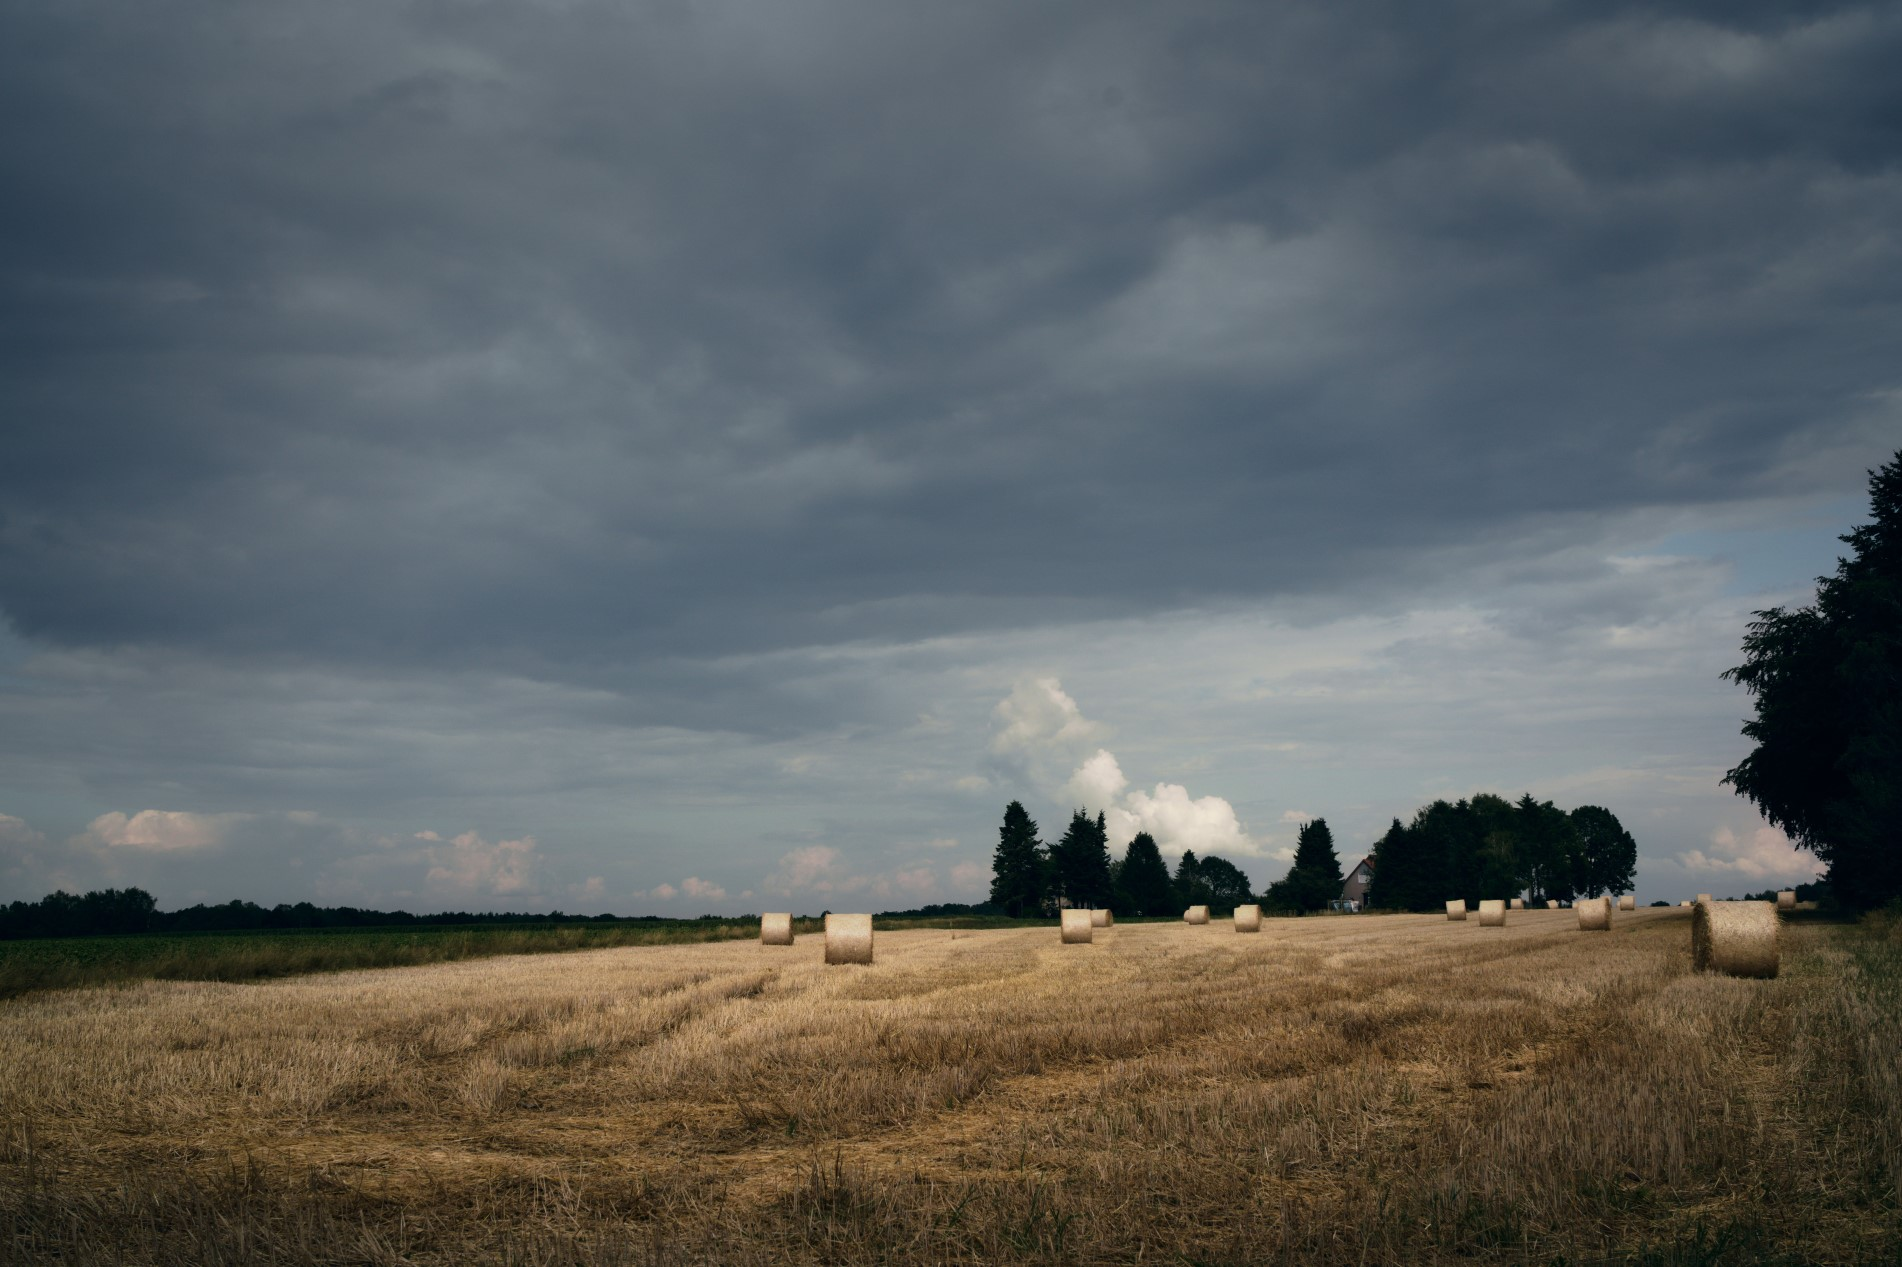
\includegraphics[width=0.5\textwidth]{field}
        }%
    }
\end{figure}

\section{Glossaries}
\label{ch:glossaries}

\ctanpackage{glossaries-extra} is an absolute unit of a package.
For this document, it is used with its back\-/end \ctanpackage{bib2gls}.
This Java tool comes with installations of TeXLive and MiKTeX.
You should already have it.
This \lcnamecref{ch:glossaries} is only a brief, opinionated overview.
For a more appropriate introduction, there is a suitable
\href{http://tug.ctan.org/macros/latex/contrib/glossaries/glossariesbegin.pdf}{Beginner's Guide},
written by the package author.
Before you jump further into the relevant, proper documentations (these are three: the
\ctanpackage{glossaries} base package, the comprehensive extension
\ctanpackage{glossaries-extra} and the helper tool \ctanpackage{bib2gls}), you might
want to give the beginner's guide a shot.

In a format similar to normal bibliographies, all glossary entries are now managed
using \texttt{*.bib} files.
Each entry is processed by \ctanpackage{bib2gls} and put into an auxiliary file.
From it, \ctanpackage{glossaries-extra} reads and inserts all contents when \verb|\gls|
and its many sibling commands are used.
The framework for all of that, also printing of the glossary and nomenclature,
is already taken care of for this document.
In addition to printing the glossaries, they are also added to the table of contents.
This behavior can be toggled using the \texttt{toc} package option flag,
see the source code for more info.

Traditionally, glossary packages are used for abbreviations.
However, using \ctanpackage{glossaries-extra} this can be kicked into top gear.
It is used for:
\begin{itemize}
    \item abbreviations,
    \item (physical) constants,
    \item symbols (greek, roman and all other),
    \item subscripts,
    \item the book index, consisting of names and the normal index.
\end{itemize}

In the case of symbols, this means the source now relies on \verb|\sym{<label>}|
commands, see also \cref{tab:available_bib_files}.
For example, equations no longer read \verb|E = mc^{2}|, but instead
\begin{verbatim}
    \sym{energy} = \sym{mass}\sym{velocity}^{2}
\end{verbatim}
This initially unintuitive approach has several critical advantages:
\begin{enumerate}
    \item absolute \textbf{consistency} following the \abb{single_source_of_truth}
        principle:
        there is exactly \emph{one} place where the symbol itself is defined.
        All other usages are just \emph{references} to this central definition.
        If suddenly, the symbol for velocity has to change from \(c\) to \(v\)
        throughout the entire document, it can be done with ease.
        Replacing single letters like that using tools like \texttt{sed} would be a
        nightmare, if not impossible.

        There is also absolutely no danger that \emph{both} symbols occur (unless
        it is explicitly set up like that), with both referring to velocity,
        as can happen when returning to a document after abandoning it for many months
        or if multiple authors work on one document.
    \item following the \textbf{\abb{what_you_see_is_what_you_mean}} principle:
        this is \LaTeX{}'s big strength.
        In the source code, it no longer states what you \emph{want to see}, but
        instead \emph{what you mean}.
        When you write \verb|E = mc^2|, you are writing what you want to see:
        the letter \texttt{E} is somehow equal to the product of letter \texttt{m}
        times \texttt{c} squared.
        But the \emph{meaning} is that \emph{energy} equals \emph{mass} times
        \emph{velocity} squared.
        This can now be expressed directly in the source code.

        The \abb{what_you_see_is_what_you_mean} principle is at the core of \LaTeX{}
        and is what sets it apart.
        It is the reason you also do not say
        \begin{verbatim}
            {\Huge\textsf{\textbf{<Section Title>}}}
        \end{verbatim}
        but instead simply
        \begin{verbatim}
            \section{<Section Title>}
        \end{verbatim}
        In the first, it was stated what the author wants to \emph{see}, but only
        in the second one does it say what was \emph{meant}.
        It is painfully obvious why the latter approach is the correct one.
        Another example is emphasized text.
        Do \emph{emphasized} (produced from \verb|\emph|) and \textit{emphasized}
        (\verb|\textit|) text look the same?
        They certainly do\dots{} usually.

        Yet, what is \emph{meant} is \emph{emphasis}; italic text is just what it
        happens to look like now, but it is not the \emph{meaning}.
        For example, we could later decide to redefine emphasized text to bold,
        or colored.
        If you previously did not differentiate strictly enough between
        \verb|\emph| and \verb|\textit|, you are in for a bad time.
        This is a trap beginners unfortunately often fall into.
        Using \ctanpackage{glossaries-extra}, abstracted markup\-/commands can be
        taken to a whole next level, leveraging this core \LaTeX{} strength.
    \item \textbf{abolishing ambiguity}:
        especially when the source code is read by other people, or even worked on,
        \enquote{naked} symbols can become ambiguous.
        What American authors refer to with a capital \emph{P}, European authors
        interpret as \emph{power}, when really \emph{pressure} was meant.
        This is a non\-/issue if in the source it says \verb|\sym{pressure}|.
        For internationalization, authors would then only adjust their
        \emph{style-sheets} (in this case the \texttt{*.bib} files) and be done.
    \item arguably improving \textbf{readability}.
        The source code can almost be read like a normal sentence consisting of full
        words, albeit with braces and backslashes in the way.
    \item printing the \textbf{nomenclature} becomes trivial.
        A single command simply prints the \texttt{*.bib} file contents.
        Being an external Java tool, the customization, sorting and filtering
        capabilities of \ctanpackage{bib2gls} for printing those lists are likely
        more than will ever be needed.
    \item lastly, some more gimmicky features are enabled, like printing all
        page numbers of occurrences of a symbol.
        Alternatively, only the first occurrence can be printed.
\end{enumerate}

\paragraph{Available Commands}
\ctanpackage{glossaries-extra} is already heavily leveraged for this document.
Take a look around the source code for all the details.
For starters, there are a couple of predefined \texttt{*.bib} files, showcased in
\cref{tab:available_bib_files}.
Note that using entries with commands like \verb|\sym{<entry name>}| is independent
of the entry type used in the \texttt{*.bib} file.
For example, subscripts are invoked using \verb|\sub{<entry name>}| despite being
defined as \verb|@symbol{<entry name> ...| in \texttt{subscripts.bib}.

\begin{table}
    \ttabbox{%
        % Brackets hold entry that will go into List of Tables (short form)
        \caption[Predefined glossaries]{%
            Predefined glossaries with their respective \texttt{*.bib} files,
            invoking commands and list occurrence in the document%
        }%
        % Use a string like 'tab:' to help with organization and auto-complete
        % when reffing
        \label{tab:available_bib_files}
    }{%
        \small
        \begin{tabular}{
            % @{<value>} specifies the column separator;
            % Use @{} to remove white space from sides (empty value)
            @{}
            *3{l}% If no other significant reason, left-align
            @{}
        }
            \toprule
                Name (\texttt{.bib}) & Command & Listed in / Description \\
            \midrule
                % \nameref is courtesy of the nameref package, which is part of
                % hyperref. It references the target by name, e.g. Chapter name.
                % However, that does not work very well for generated chapter names.
                \texttt{terms} & \texttt{\textbackslash idx} & Index \textrightarrow{} Terms \\
                \texttt{names} & \texttt{\textbackslash name} & Index \textrightarrow{} Names \\
            \addlinespace
                \texttt{roman} &
                    \texttt{\textbackslash sym} &
                    \nameref{ch:glossary} \textrightarrow{} Symbols \textrightarrow{} Roman \\
                \texttt{greek} &
                    \texttt{\textbackslash sym} &
                    \nameref{ch:glossary} \textrightarrow{} Symbols \textrightarrow{} Greek \\
                \texttt{other} &
                    \texttt{\textbackslash sym} &
                    \nameref{ch:glossary} \textrightarrow{} Symbols \textrightarrow{} Other \\
            \addlinespace
                \texttt{subscripts} &
                    \texttt{\textbackslash sub} &
                    \nameref{ch:glossary} \textrightarrow{} Subscripts \\
            \addlinespace
                \texttt{constants}\mpfootnotemark[1] &
                    \texttt{\textbackslash cons} &
                    \nameref{ch:glossary} \textrightarrow{} Numbers \\
            \addlinespace
                \texttt{abbreviations} &
                    \texttt{\textbackslash abb} &
                    \nameref{ch:glossary} \textrightarrow{} Acronyms \\
            \bottomrule
        \end{tabular}
        \footnotetext[1]{%
            Constants like \cons{pi} are toy examples for this document.
            However, this glossary section is very convenient to share assumptions
            and used constants in a clear and concise way in one central place,
            aiding reproducibility and overall document integrity.%
        }
    }%
\end{table}

\paragraph{Modifying Print Output}
To use glossary entries but not print them in a glossary, comment out the entire
relevant \verb|\printunsrtglossary| macro where appropriate.
For the index, the relevant command is \verb|\printunsrtindex|.
Some glossary categories, like \emph{Symbols}, have sub\-/categories, like \emph{Roman},
\emph{Greek} and \emph{Other}.
To omit printing a single sub\-/category in the glossaries (but still allow their use
in the document%
\footnote{
    The \emph{Other} symbol entries are required for the provided built\-/in math
    macros, see \cref{tab:predefined_math_macros}, to work!%
}%
), refer to the \texttt{notprinted} type and the instructions found in the \texttt{*.cls}
file.

\subsection{bib2gls}
\label{ch:bib2gls}

\ctanpackage{bib2gls} is an external tool (of the same name as the package) that
\ctanpackage{glossaries-extra} employs to convert external \texttt{*.bib} files with
definitions for, for example, acronyms, into a \TeX{}\-/compatible format.
During conversion, it also processes all the entries, like sorting them in whatever
way you request.
The sorting and filtering capabilities are very strong, and of course also Unicode
compatible.
A minimal \texttt{bib} file for acronyms can be as simple as:
\begin{minted}[linenos=false]{bib}
    @abbreviation{cont_int,
        short={CI},
        long={Continuous Integration},
    }
\end{minted}
For concrete examples, see the files for this document at \texttt{bib/glossaries/}.
There can be as many keys as required, with custom ones being easily created.
Effectively, this is analogous to how bibliography entries are created.
Thus, users of \LaTeX{} who are already familiar with that concept and format
should have an easy time getting started with \ctanpackage{glossaries-extra}.
Using it for mathematical symbols can look like:
\begin{minted}[linenos=false]{bib}
    @symbol{abs_temperature,
        name={\ensuremath{T}},
        description={absolute temperature},
        group={roman},
        unit={\si{\kelvin}},
    }
\end{minted}

\begin{landscape}
    \section{Landscape}

    Pages in landscape format are rather straightforward to implement.
    Note that not only are these in landscape orientation; they are also recognized
    as such by supporting document viewers, rotating the page for you and keeping
    it legible.
\end{landscape}
